\section{Résumé}
Notre équipe ayant été séléctionée parmi un grand ensemble d'autres équipes afin de confectionner le meilleur de la technologie spatiale embarquée en partant d'un Raspberry Pi, toute l’ambition de "The Astronogame©" est de parvenir à transporter des informations et/ou messages dits « classés secret-défense », tels des codes d’entrées d’installations nucléaires, de palais royaux ou encore de lieux publiques sensibles, eux aussi, démunis face à une éventuelle menace.\\
C'est avec toute cette technologie embarquée que nous avons dû travailler.\\

\newline
Pour rappel, les objectifs principaux furent :
\begin{description}
    \item [1 :] Proposer un menu exploitant chacune des facultés de l'appareil (LED, (SenseHat), Joystick).
    \item [2 :] Le message devait être composé d’une suite de chiffres de 0 à 9, entrés directement sur le MagicLock grâce à l’interface. Attention, si message il y a, l'utilisateur doit avoir la permission de voir ou supprimer le message une fois le code correctement saisi. Si rien n'est stocké dans le Pi, l'utilisateur doit avoir la possibilité d'enregistrer un message.
    \item [3 :] Le code doit être une suite de positions du Raspberry PI et du Sense Hat dans l’espace (à plat, gauche, droite, ...) et ce dans les 3 dimensions de l’espace avec après chaque position dans la séquence une validation par un appui sur le Joystick.
    \item [4 :] Le message et le code devaient être conservés sous formes de fichiers, et être de nouveau disponibles en cas d’extinction du Raspberry PI et de remise sous tension.
    \item [5 :] Le message devaitt être conservé sous forme chiffrée, et le code quant à lui sous forme hachée.
\newline
\newline
\end{description}

Ayant voulu voir plus loin que les conditions minimes données, nous avions eu tellement d'idées que nos tuteurs ont jugé notre projet trop "ambiteux" par rapport au temps qui nous était offert... Et bien, c'est avec joie que l'on peut vous affirmer que nous sommes parvenus à créer un programme stable, respectant le contrat de base et bien sûr remplis d'extensions (très) originales et à couper le souffle.
N'ayant pas eu assez de maîtrises pour gérer le "Multi-Tasking" et donc la gestion de plusieurs fichier ".py" en même temps, l'ensemble du code se trouve dans un seul fichier, appelé "main.py" et comporte ainsi plus de 2000 lignes ! Ca promet, n'est-ce pas ?
\newline

\section{Déroulement du système}
Même si certaines conditions MINIMES sont imposées, nous sommes très enthousiaste à l'idée de proposer aux utilisateurs des fonctionnalitées plus poussées ou amusantes. Après des heures de réunions, l’équipe travaillant sur le projet, s’est enfin mise d’accord sur un système de chiffrement révolutionnaire et inviolable…
\newline\newline
Tout d'abord, une fois le Raspberry Pi allumé pour la première fois, cet engin vous semblera normal : en effet un menu contrôlable à l'aide du Joystick vous permettra de vous voyager à travers ce dernier et ainsi vous affichera les 4 jeux disponibles :
\begin{description}
    \item [Guitar Hero :] Affiche une série de direction "random" sur l'écran... l'utilisateur n'a qu'à reproduire ces directions via le Joystick.
    \item [Donkey Kong :] Un ensemble de tonneaux ne cessent de tomber au dessus de votre tête... Parviendrez-vous à atteindre de l'autre coté ?
    \item [Labyrinth V1 :] Il s'agit d'un simple labyrinthe 8x8 pixels avec un pion (vous) et un objectif. Il est contrôlable via le Joystick OU via l'accéleromètre (nécessite après chaque mouvement un appui du Joystick).
    \item [Labyrinth V2 :] Il s'agit ici, en revanche, d'un labyrinthe beaucoup plus complexe : en effet, l'utilsateur devra faire face ici non pas à un labyrinthe 8x8 pixels mais bien 64x64 pixels ! A l'aide de téléporteur et de votre débrouillardise, parviendrez-vous à atteindre l'objectif ? Ce jeu est lui aussi contrôlable via le Joystick OU via l'accéleromètre (nécessite après chaque mouvement un appui du Joystick).
\end{description}
\newpage
C'est ici que les choses deviennent plus intéressantes : C'est objet étant réservé aux agents secrets, il est bien clair que le Raspberry n'affiche pas que de simples jeux...Il contient également un menu secret ! Pour le faire apparaitre c'est très simple (ou presque). Il suffit que l'agent secret rentre un mot de passe. Ce mot de passe, qui est une combinaison de 6 mouvements dans l'espace et prédéfini par 6x l'appareil à plat, fera uniquement si la combinaison est bonne, apparaitre un logo de chargement en forme de clé et ensuite, TADAAAAM : le fameux menu secret ! Ce menu secret correspond aux attentes principales de nos supérieurs, à savoir :
\begin{description}
    \item [See :] Permet de voir le message écrit par l'agent secret.
    \item [Edit :] Modifier ou écrire un message.
    \item [Delete :] Pour supprimer le message.
    \item [Password Editor :] Donne la possibilité à l'agent secret de modifier son mot de passe pour entrer dans le menu secret.
    \item [Exit :] Sortir du menu secret et revenir ainsi dans le menu des jeux.
\end{description}
Il faut bien entendu savoir que le message enregistré sera conservé sous forme hachées, c'est-à-dire presque indécryptable par la récupération externe de fichier.
Le code sera lui conservé sous forme cryptée.
\newline
\newline
Mais ce n'est pas tout ! Voulant pousser la sécurité au plus loin, nous avons décider d'ajouter à tout cela 3 extensions majeures : 
\begin{description}
    \item [Access Level© :] Lors de la création d'un message, une fois celui-ci sauvegardé, notre système proposera à l'utilisateur de choisir un niveau d'accréditation allant de 0 à 5. Une fois le niveau choisi, lorsque l'utilisateur voudra voir/ modifier ou supprimer le message, un jeu/énigme lui sera proposé en fonction du niveau précédemment choisi.
    \newline
    Les niveaux d'accréditation sont définis comme suit :
\begin{description}
    \item [Niveau 0 :] Aucune action requise.
    \item [Niveau 1 :] Le système proposera une énigme simple à résoudre afin de vérifier les connaissances de l'agent.
    \item [Niveau 2 :] Le système proposera le labyrinthe V2.
    \item [Niveau 3 :] Le système proposera Guitar Hero.
    \item [Niveau 4 :] Le système proposera le Donkey Kong + une énigme.
    \item [Niveau 5 :] Le système proposera le labyrinthe V2.
\end{description}
    \item [Fast Delete© :] Imaginons vous êtes l'agent secret et vous avez un message qui a pour niveau d'accréditation 5. Un espion vous attaque par surprise et veut à tout prix récupérer le message que contient la machine, vous allez cliquer sur supprimer et vous amusez à faire le labyrinthe 64x64 pixels ? Vraiment ? Bine sûr que non : Une autre combinaison, qui est définie de base par 6x plat elle aussi, peut se faire si vous vous trouvez sur le logo "Delete" du menu secret. Ainsi, pas besoin de vous amusez à jouer et vous pouvez mourir tranquile ! (Cette combinaison est elle aussi modifiable via le "Password Editor".)
    \item [Back Up© :] Si jamais l'utilisateur rate 3 fois l'Access Level©, le message sera automatiquement supprimé et il lui sera impossible de le voir. Seulement, si par malheur le 3 essais du jeu ne lui ont pas suffit et veut à tout pris récupérer le message, une solution est possible : une fois sur le logo "See" du menu secret, il devra tout simplement faire la combinaison Fast Delete© sur ce logo et ainsi un message "Message restored" apparaitra !
\end{description}
\newpage

\section{Planning}
\begin{center}
    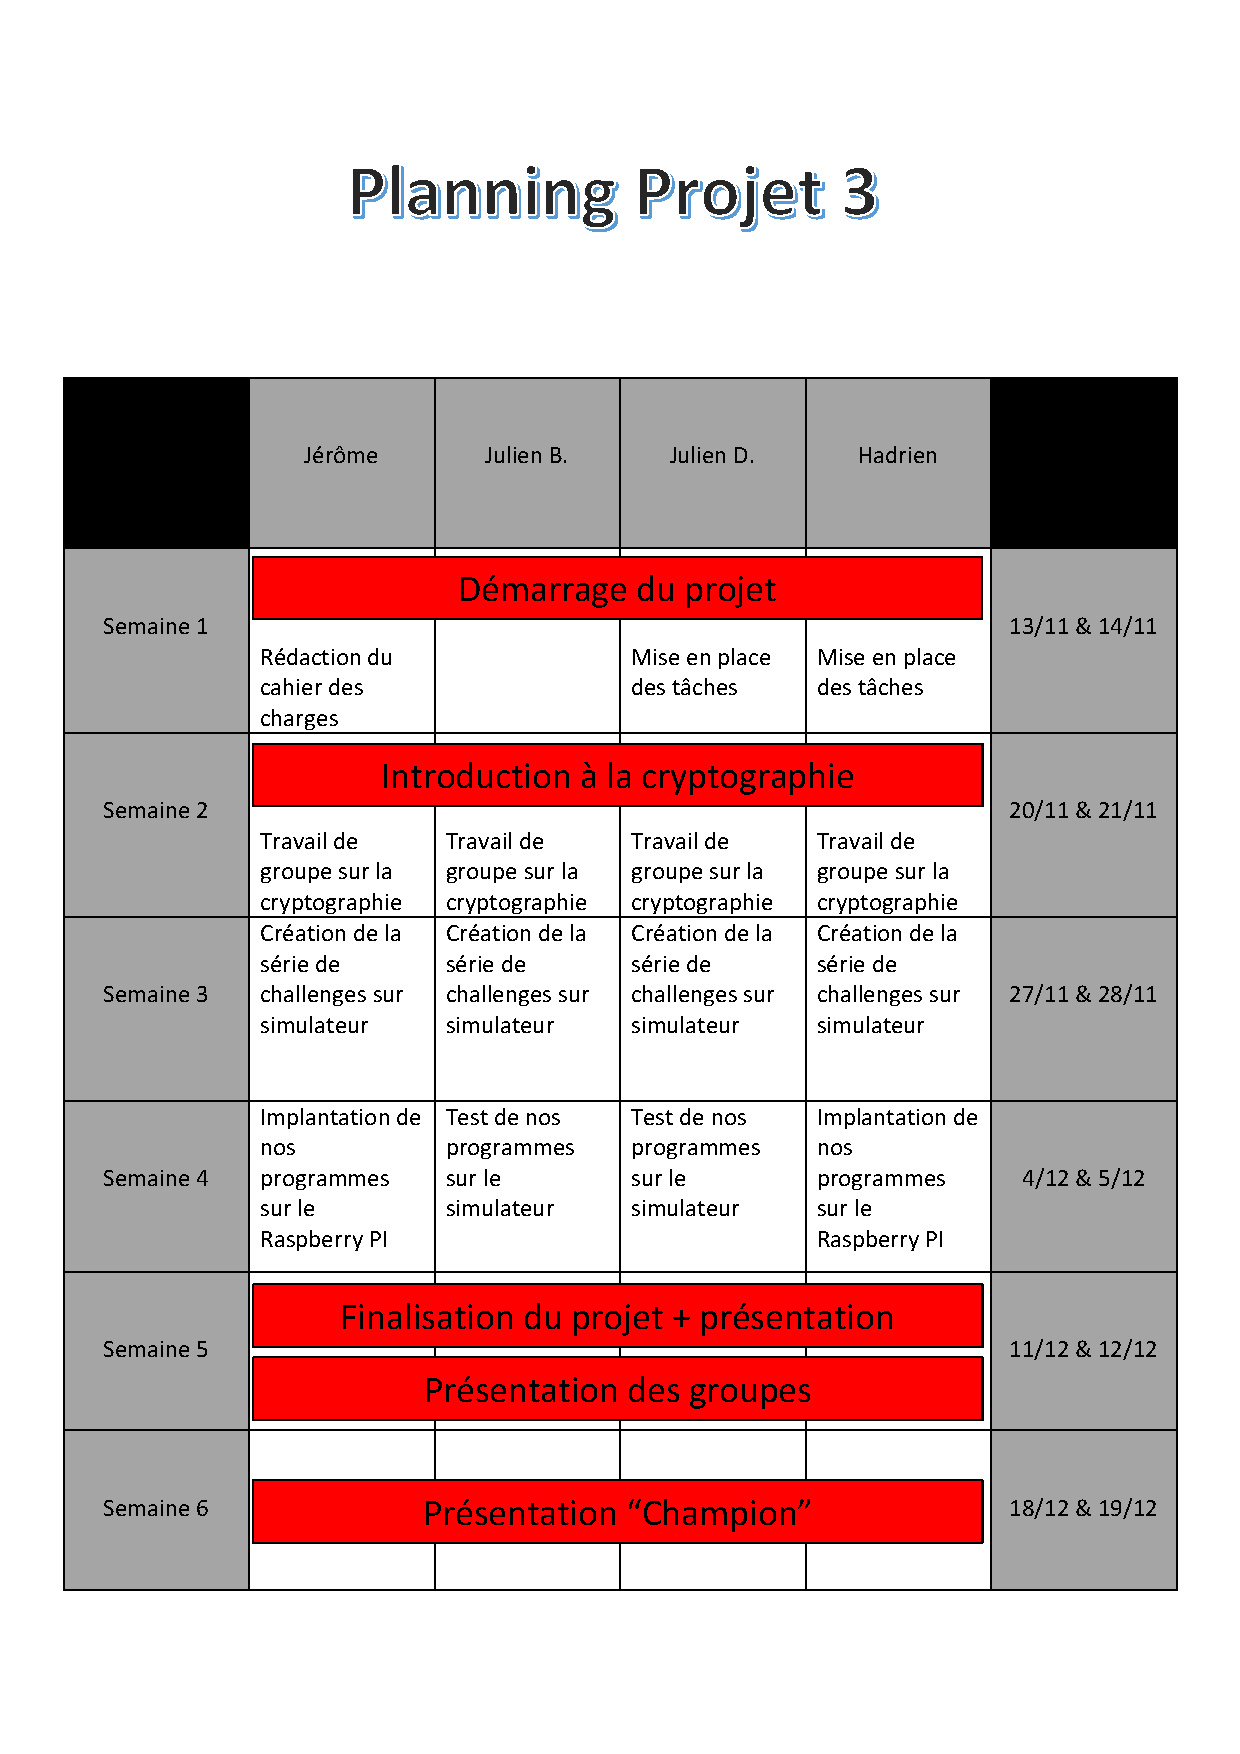
\includegraphics[width=12cm]{PlanningP3.pdf}
\end{center}

\section{Conclusion}
Ceci conclut donc notre premier quadrimèstre... Nous pouvons dire que ce dernier projet de l'année civile nous a vraiment tenu à coeur : envie et jusqu'au-boutisme nous ont permis d'aller très loin et d'être d'ailleurs parmis les chanceux pour se présenter devant un jury externe. Ce groupe fut au final une bande de potes voulant à tout prix gagner et montrer en quoi l'électronique et l'informatique peuvent faire de belles choses. Durant ces mois de travail très peu de problèmes ont été rencontré... Le plus gros fut le gyroscope. Il falalit en effet utilisé l'accéleromètre et non ce dernier. Ceci termine ce projet 3.  